\section{پیاده‌سازی و تنظیمات}

در این بخش، ابتدا نحوه استفاده از داده ها را میبینیم. سپس نگاهی به فرمت و خود فایل تنظیمات (\lr{Config file}) میکنیم و به صورت خیلی کوتاه کد را بررسی میکنیم و در نهایت خروجی کد را برای تنظیمات $default$ آن میاوریم. 

\subsection{داده های CSV}

در بخش اول، دیدیم که میتوانیم فایل های 
\lr{.pcap}
را تمیز کرده و داده های مورد نیازمان را از آنها استخراج کنیم و به صورت 
\lr{.csv}
در بیاوریم. 

اگر این داده ها را باز کنیم، ستون هایمان این ها میشوند:

\begin{figure}[h]
	\centering
	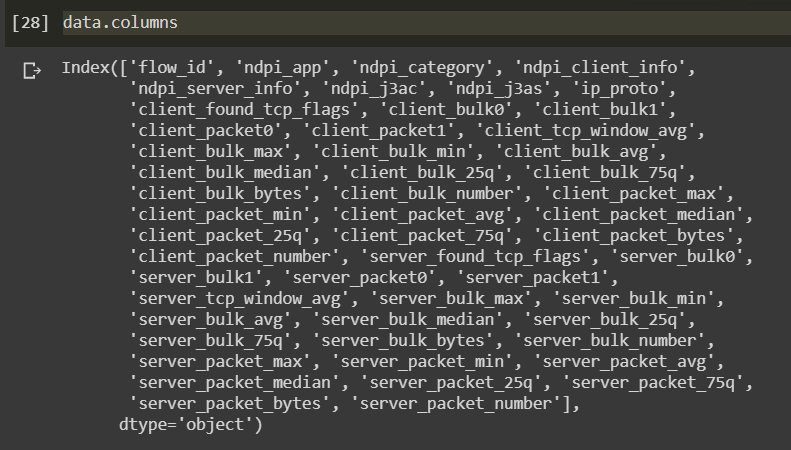
\includegraphics[width=0.6\textwidth]{training/6}
	\caption{ستون‌های داده}
	\label{fig:training:data-columns}
\end{figure} 


که در بین اینها، ستون 
\lr{ndpi-category}
همان چیزی است که ما به دنبال یافتنش هستیم. در واقع 
\lr{label}
هایمان، ستون 
\lr{ndpi-category}
است و بقیه ستون ها، ورودی هایمان با مدل ها است. 

این ستون 6 مقدار متفاوت دارد. این مقادیر را میتوان در عکس زیر دید:
\begin{figure}[h]
	\centering
	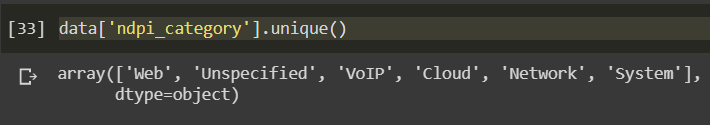
\includegraphics[width=0.6\textwidth]{training/7}
	\caption{مقادیر \lr{label} ها}
	\label{fig:training:class-labels}
\end{figure} 
 که این مقادیر را در ادامه در هنگام مشاهده نتایج، دوباره میبینیم.
 

\subsection{فایل تنظیمات و کد} 
حالا برمیگردیم به خود کد که مدل های مختلف را اجرا میکند. این کد در فایل 
\lr{evaluate\_classifiers.py}
قرار دارد. نحوه عملکرد کد به این صورت است که یک فایل تنظیمات که به فرمت 
\lr{.yaml}
است در ورودی میگیرد که در آن، تنظیمات تمامی مدل هایی قرار دارد که میخواهیم بررسی‌شان کنیم. سپس بر اساس تنظیماتی که در فایل آمده، مدل های خود را ساخته و عملیات یادگیری را انجام میدهد. و در نهایت مجموع تمامی نتایج بدست آمده را چاپ میکند. میتوان بخشی این فایل تنظیمات را در زیر دید:

\begin{figure}[h]
	\centering
	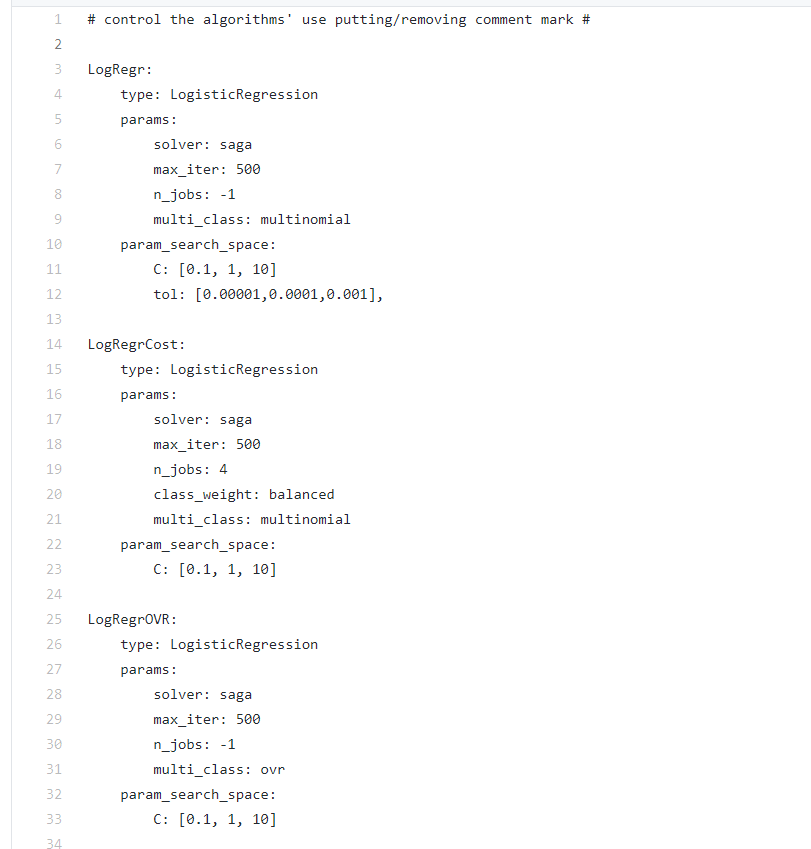
\includegraphics[width=0.6\textwidth]{training/8}
	\caption{فایل تنظیمات}
	\label{fig:training:config-file}
\end{figure} 

همانطور که میبینید، در مورد اول، از 
\lr{Logistic Regression}
میخواهد استفاده کند و میخواهد تمامی حالاتی که پارامتر $C$ اش از بین 
$[0.1, 1, 10]$
انتخاب شود و پارامتر  $tol$ اش از بین 
$[0.00001,0.0001,0.001]$
انتخاب شده است را بررسی کند. در این کد، تمامی مدل ها توسط کتابخانه $sklearn$ پیاده‌سازی شده است و کافی است برای یادگیری آنها، پارامتر هایشان ست شوند و داده ها را به عنوان ورودی با آنها بدهیم و تابع $fit()$ را رویشان صدا بزنیم. 

مشابه همین تنظیمات، برای انواع مدل های دیگر وجود دارد. 

\subsection{نتایج اجرا}

با دادن این فایل کانفیگ به عنوان ورودی به کد، تمامی حالات مختلف اجرا شده و بهترین نتایج نمایش داده میشوند. در زیر میتوان خلاصه نتایج پس از اجرای کد را دید:

\begin{figure}[h]
	\centering
	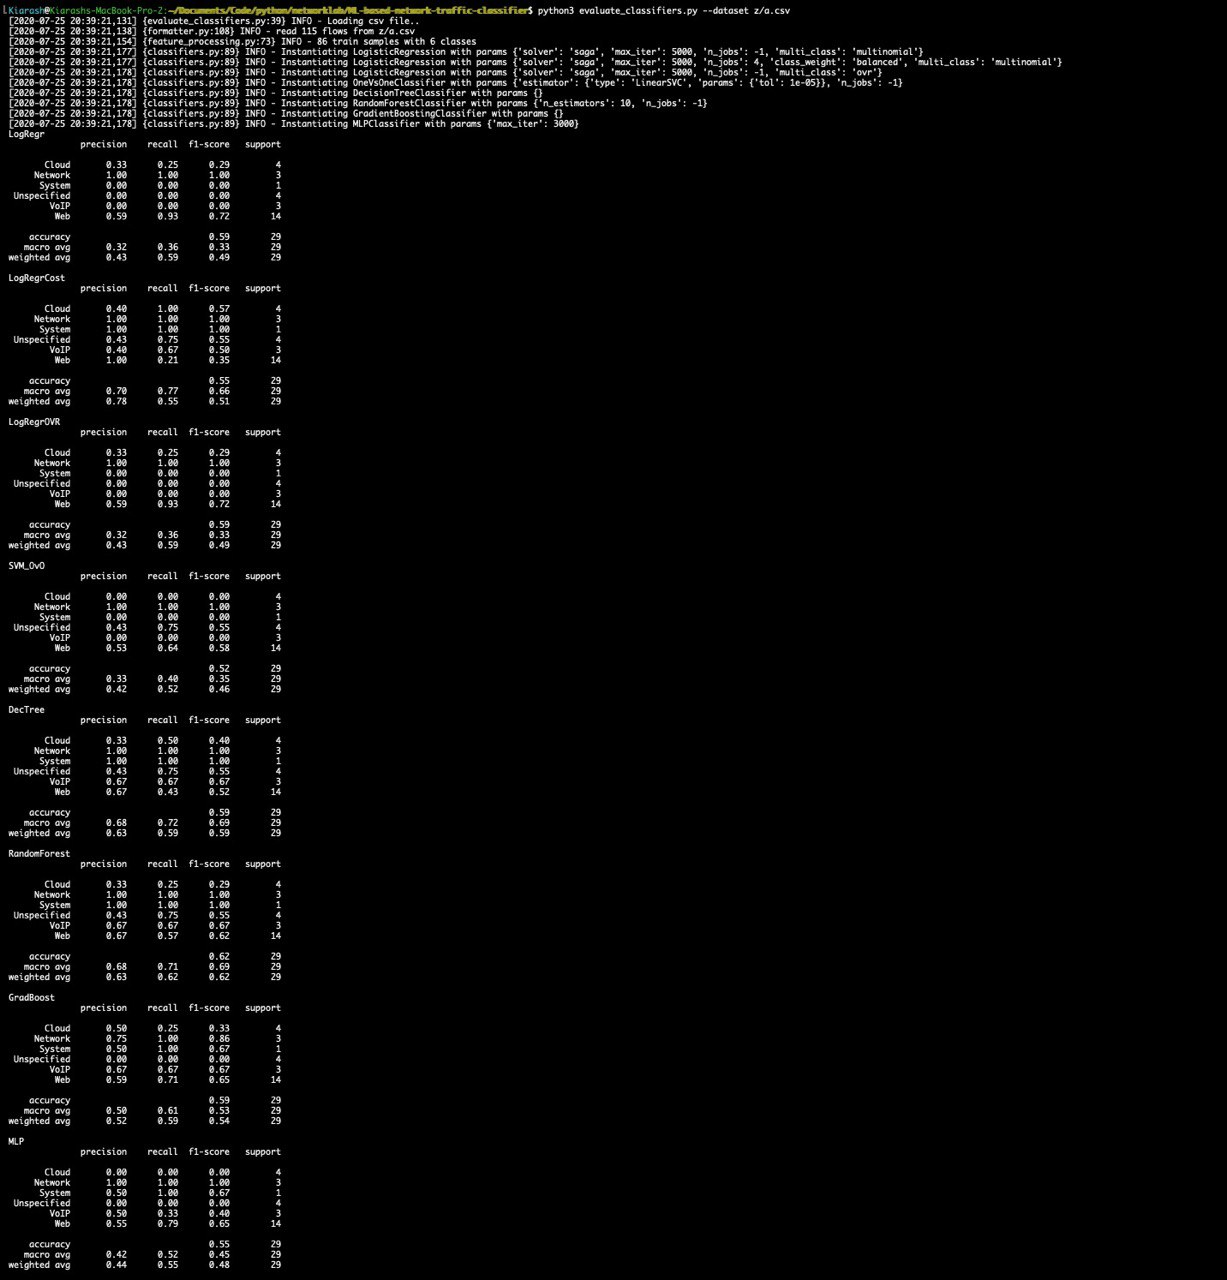
\includegraphics[width=0.9\textwidth]{training/9}
	\caption{نتایج اجرا}
	\label{fig:training:results}
\end{figure} 

در اینجا، همانطور که دیده میشود، متریک های متفاوت برای هر کلاس در هر مدل آورده شده است. به عنوان مثال میتوانیم ببینیم که مدل 
\lr{Random Forest}
مان روی کلاس های مختلف حداقل 
\lr{33\%}
 و حداکثر
\lr{100\%}
 دقت پیدا کرده است. 
